\chapter{ Le modele standard } \label{ch:introduction_physique}

Cette thèse s'inscrit dans le cadre du modèle standard de la cosmologie.
Ce modèle considère un univers en expansion $\Lambda$ composé essentiellement de matière noire froide (Cold Dark Matter) $\Lambda$ Cold Dark Matter ($\Lambda$CDM)

L'idée d'un univers non statique a pris forme dans le début du XIX eme siècle suite a deux evenement majeurs, d'un coté l'élaboration de la théorie de la relativité générale d'Einstein en 1915 a permis la mise en place d'un cadre theorique propice, et d'un autre coté, plus d'une decenie plus tard les observation de Hubble entre 1923 et 1929.

\section{Loi de Hubble ( observation) }

Hubble observe deux phenomème qui vont mené a une redeffinition de notre notion de cosmologie.
Il est le premier a observer qu'il existe d'autre galaxie que la voie lactée.
De plus il observe une relation entre la distance de ces nouvelles galaxies et leurs spectre lumineux.
Plus ces galaxies sont  éloignées, plus leurs spectre et décalé vers la rouge.
Il interpretat ce décallage comme un effet dopler et montra que ces galaxie s'éloigne de l'observateur.

\begin{figure}[bth]
        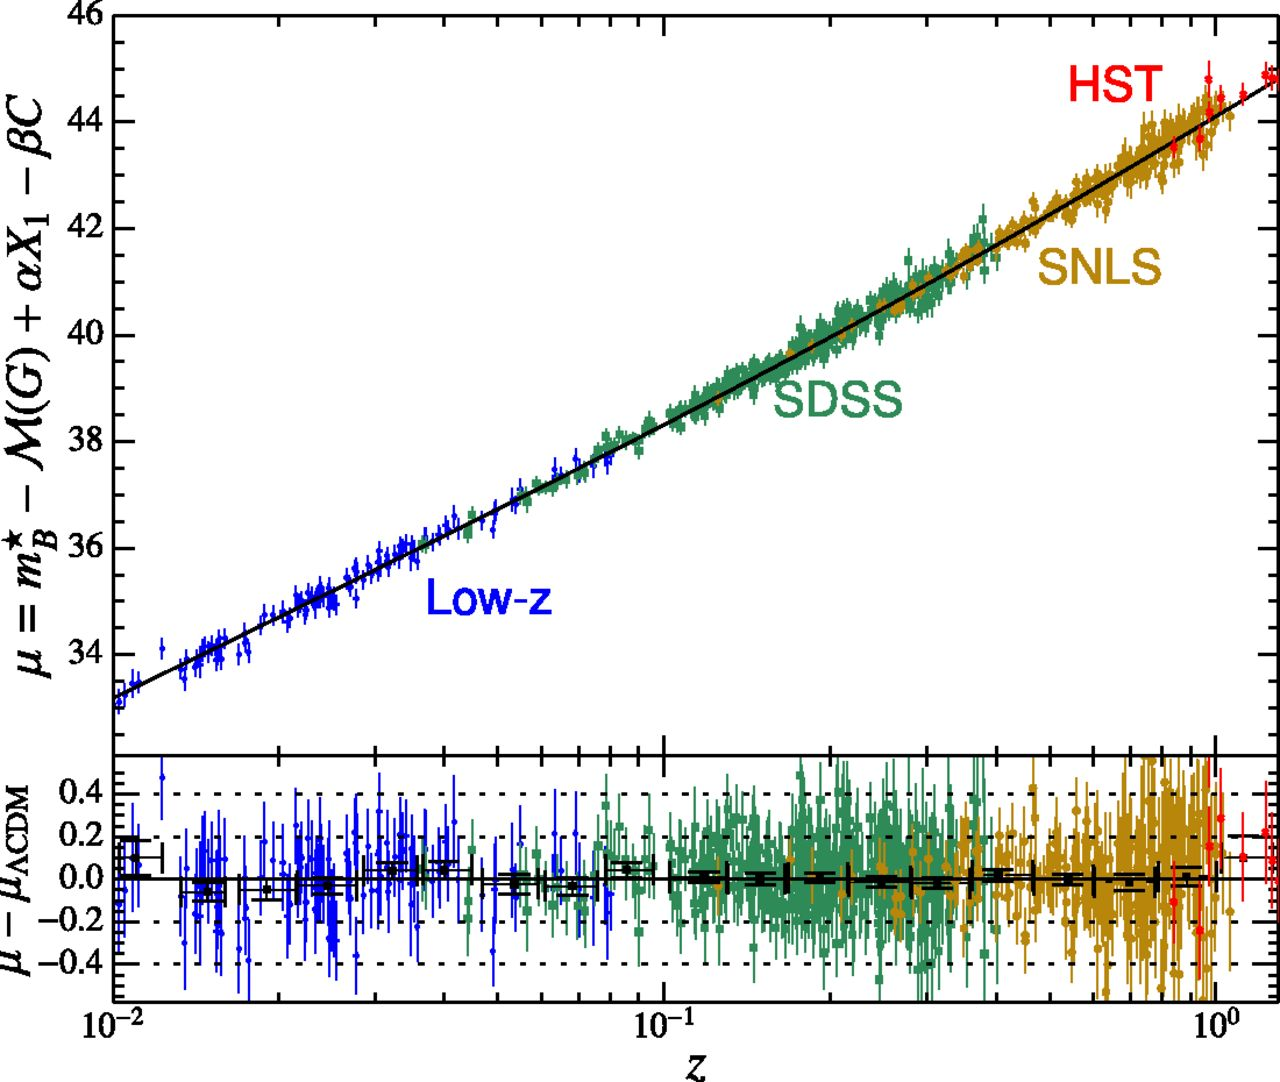
\includegraphics[width=.9\linewidth]{img/01/hubble_law.jpg} 
        \caption{Loi de Hubble a partir d'observation actuelles. 
%http://www.pnas.org/content/112/11/3173/F2.expansion.html
        Image ESO}
 		\label{fig:hubble_law}
\end{figure}

Cette relation entre la distance des galaxies $D$ et leurs vitesse d'éloignement $V$ est aujourd'hui appelée loi de Hubble et peux etre résumé par :

\begin{equation}
V = H_0 D, 
\end{equation}
 ou $H_0$ est la constante de Hubble.

Cette correlation est aujourd'hui tres bien etablie observationelement (Fig. \ref{fig:hubble_law})

Ces observations on permis de confirmer ce qui avait été pressentis par Einstein plus d'une decenie plus tot, lorsqu'il introduisit le concept de constante cosmologique (qu'il nomma $\Lambda$). 
Ce concept 


découverte des galaxies\\
découverte de l'expansion de l'univers


\begin{figure}[bth]
        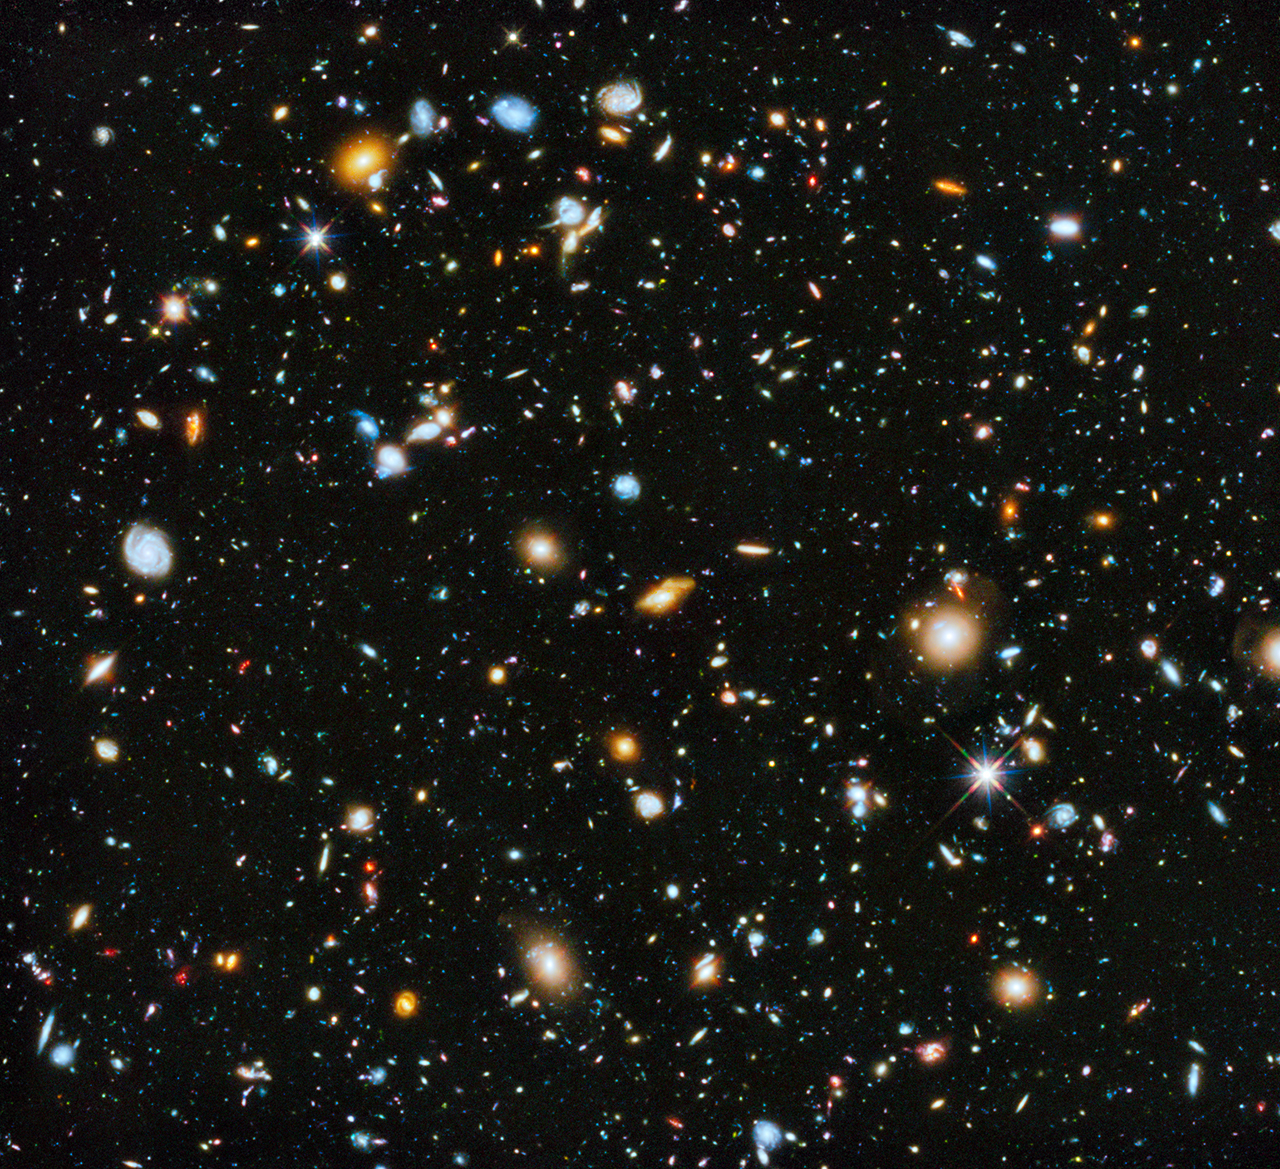
\includegraphics[width=.9\linewidth]{img/01/hudf.jpeg} 
        \caption{Hubble Ultra Deep Field 2014. 
        Image NASA}
 		\label{fig:hubbl_deep_field}
\end{figure}

\section{théorie - lCDM}

le big bang\\
l'inflation\\
la nucléosynthèse\\
le CMB\\
la reionization


\section{Le CMB}


\subsection{Observations}

Penzias et Willson

\subsection{Théorie}

surface de dernière diffusion


\subsection{Température}
Le cosmic Microwawe background se presente sous la forme du corp noir le plus parfait connus.
Fig. \ref{fig:cmb_thermal_spectrum}
T=2.73K


\begin{figure}[bth]
        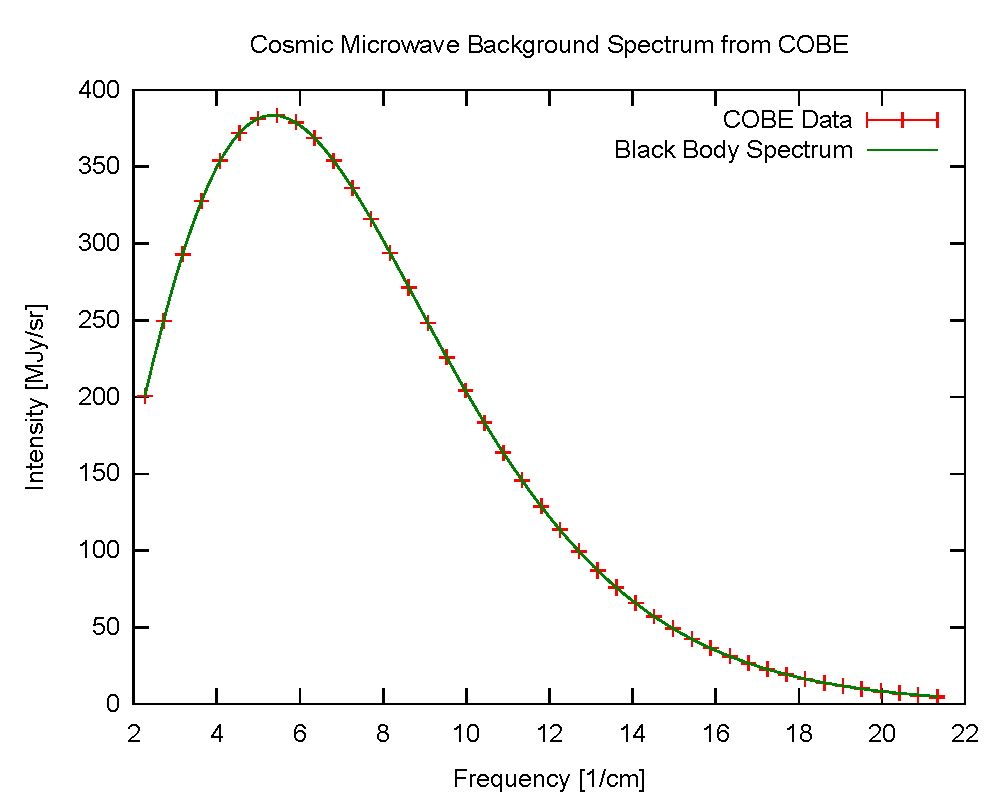
\includegraphics[width=.95\linewidth]{img/01/Cmbr.pdf} 
        \caption{Spectre thermique du CMB vue par le satellite Cosmic Background Explorer (COBE). 
        Image Wikipédia}
 		\label{fig:cmb_thermal_spectrum}
\end{figure}




\subsection{Spectre de puissance}

Le CMB n'est pas uniforme, il presente de tres faibles fluctuations (1e-5)qui nous renseigne sur l'etat de l'univers au moment de son emission.
Fig. \ref{fig:cmb_power_spectrum}

\begin{figure}[bth]
        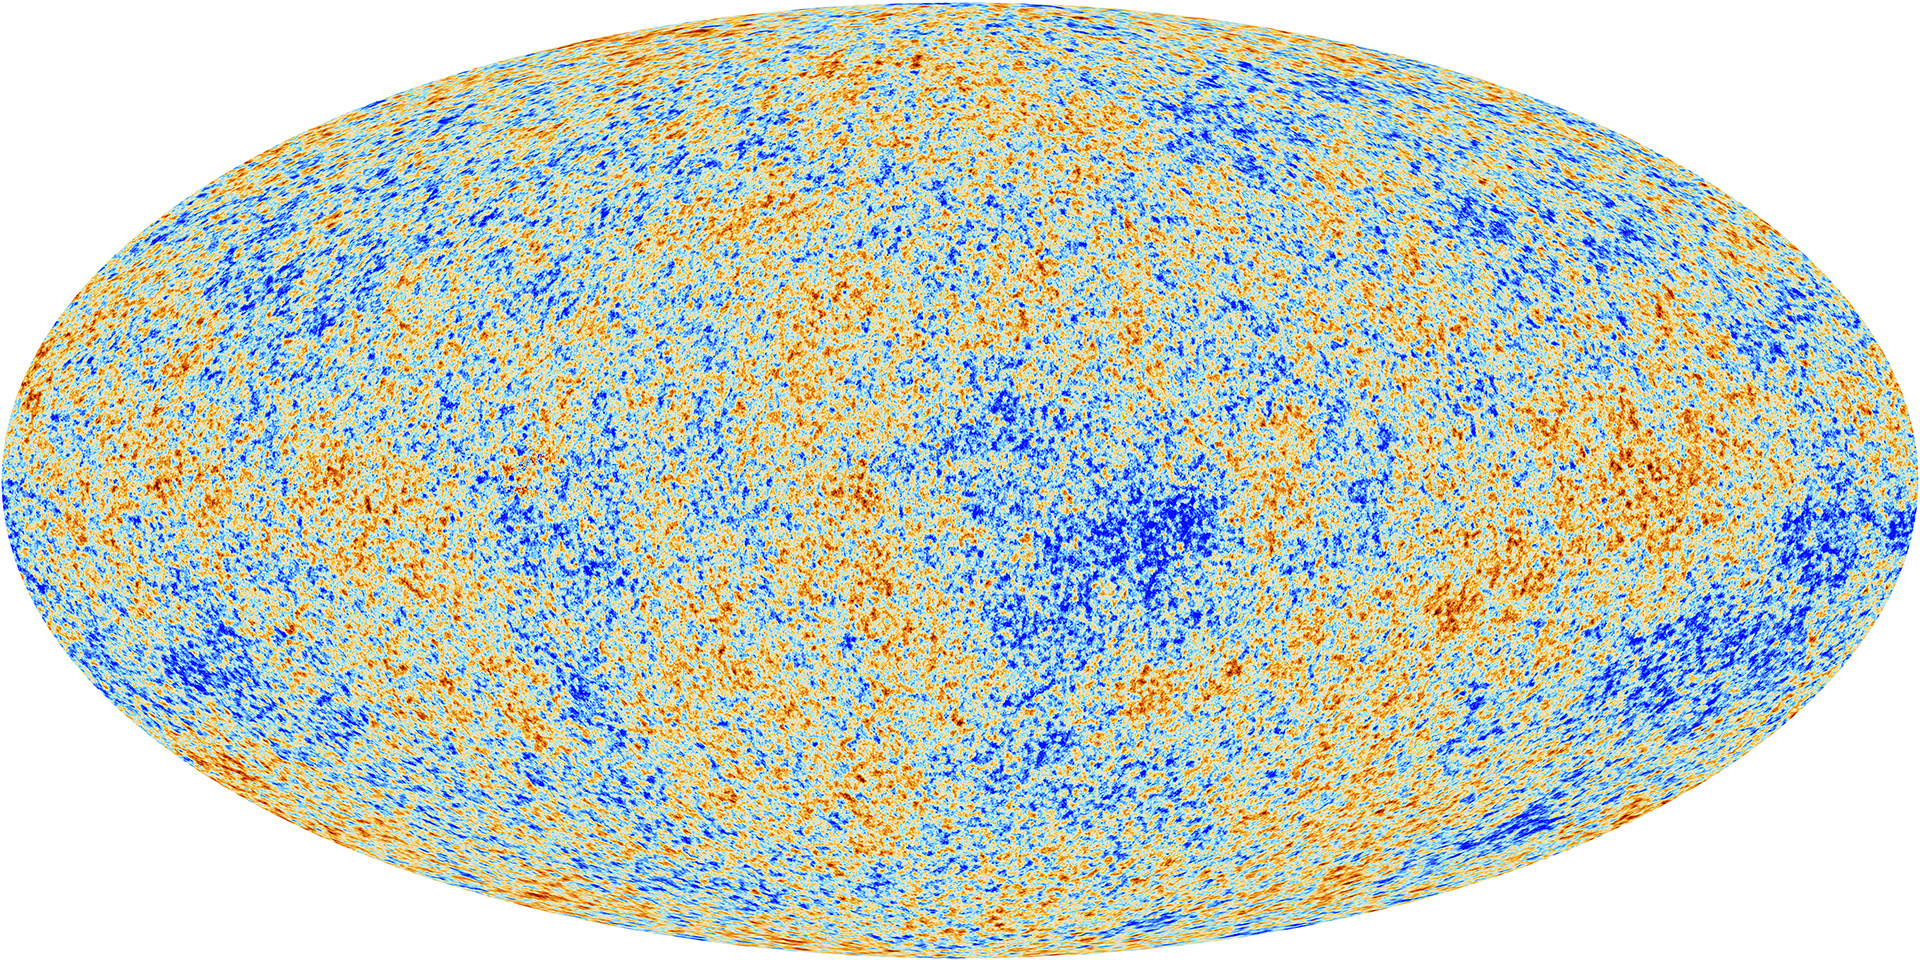
\includegraphics[width=.95\linewidth]{img/01/CMB.jpeg} 
        \caption{Les fluctuation du CMB vues par le satellite Planck. 
        Image ESA}
 		\label{fig:cmb}
\end{figure}


En decomposant ces fluctuations en harmoniques sphériques:
Fig\,\ref{fig:harmoniques_spheriques}

decomposition en multipoles
%https://www.physicsforums.com/threads/can-someone-explain-angular-power-spectrum.309483/
\begin{equation}
 \frac{\Delta T(\theta,\phi)}{T} = \sum_{l>0} \sum_{m=-l}^l a_{lm} Y(\theta,\phi)_{lm}
\end{equation}

avec : 

\begin{equation}
a_{lm}= \int d\Omega(\theta,\phi) \Delta T (\theta,\phi) Y(\theta,\phi)_{lm}
\end{equation}

\begin{figure}[bth]
        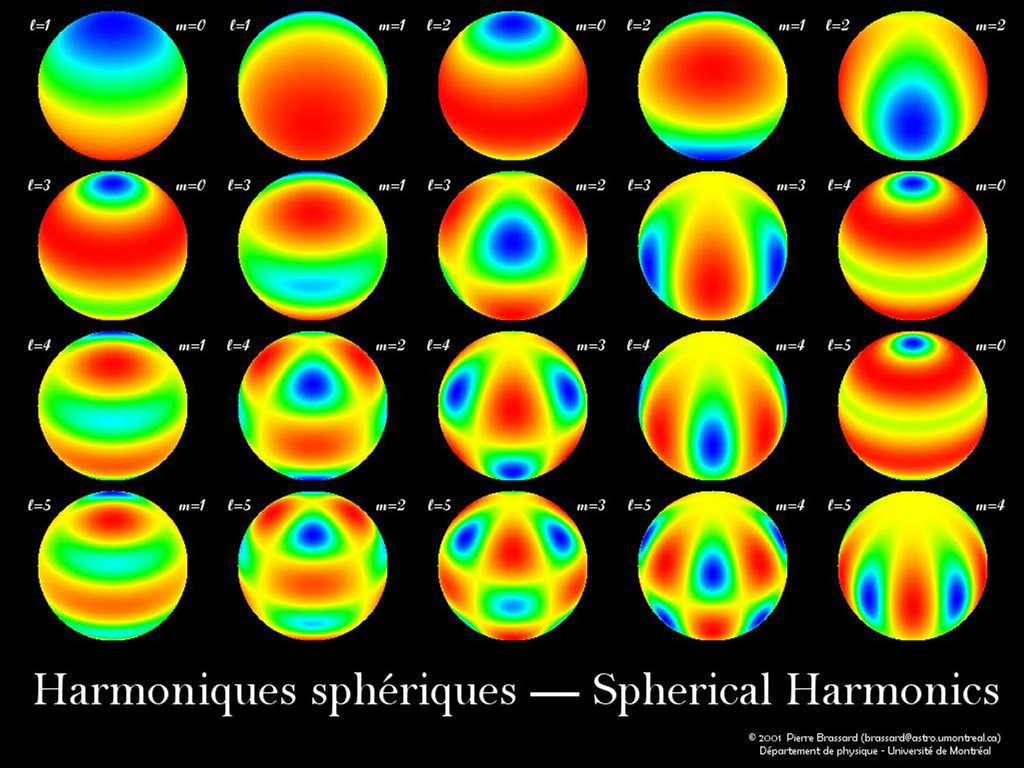
\includegraphics[width=.95\linewidth]{img/01/harmoniques_spheriques.jpeg} 
        \caption{
        représentation des $Y(\theta,\phi)_{lm}$
 Pierre Brassard, université de Montréal 
%Spectre thermique du CMB vue par le satellite Cosmic Background Explorer (COBE). 
        Image Wikipédia}
 		\label{fig:harmoniques_spheriques}
\end{figure}


\begin{equation}
C_l = \frac{1}{2l+1} \sum_{m=-l}^l a_{lm} a_{lm}^*
\end{equation}


Et finalement, on obtient le spectre de puissance:

\begin{equation}
D_l = \frac{l (l+1) C_l }{2 \pi} 
\end{equation}

représenté Fig.\,\ref{fig:cmb_power_spectrum}

\begin{figure}[bth]
        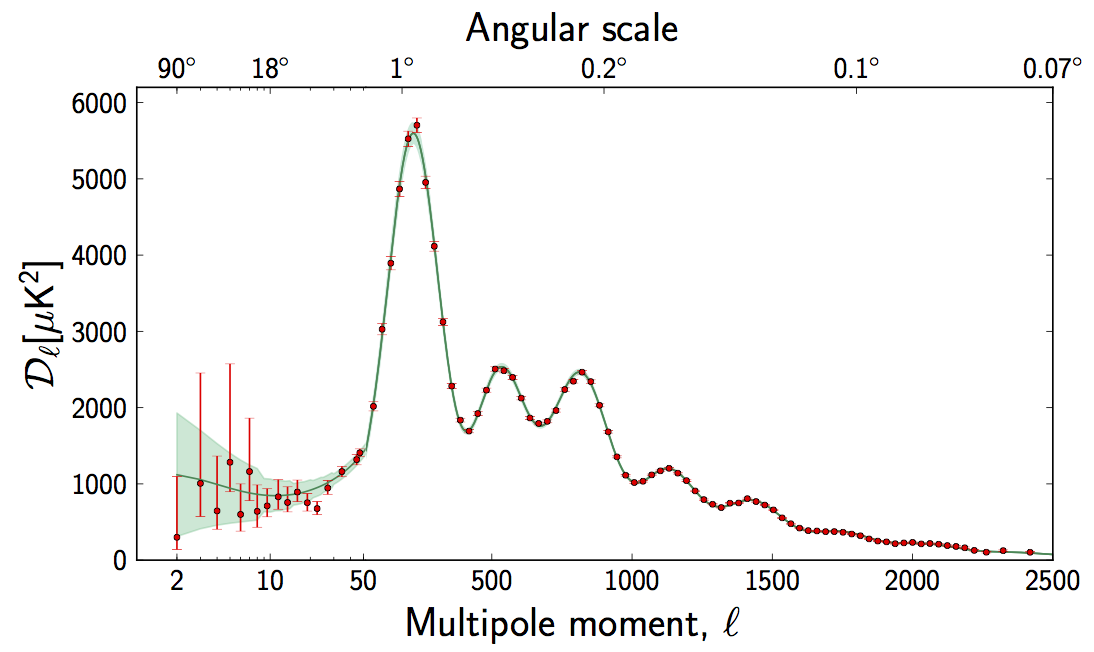
\includegraphics[width=.95\linewidth]{img/01/CMB_power_spectrum.png} 
        \caption{Spectre de puissance des fluctuation du CMB.
        Image ESA}
 		\label{fig:cmb_power_spectrum}
\end{figure}


\section{Le contenu de l'univers - (Théorie)}

Pour simuler l'univers, on a besoin de savoir ce qu'il contient. 
A partir du spectre de puissance, on peut déterminer les différentes composantes de l'univers (paramètres cosmologique).

univers infini, homogène, isotrope


%https://ned.ipac.caltech.edu/level5/Freedman2/Freed6.html


\begin{figure}[bth]
        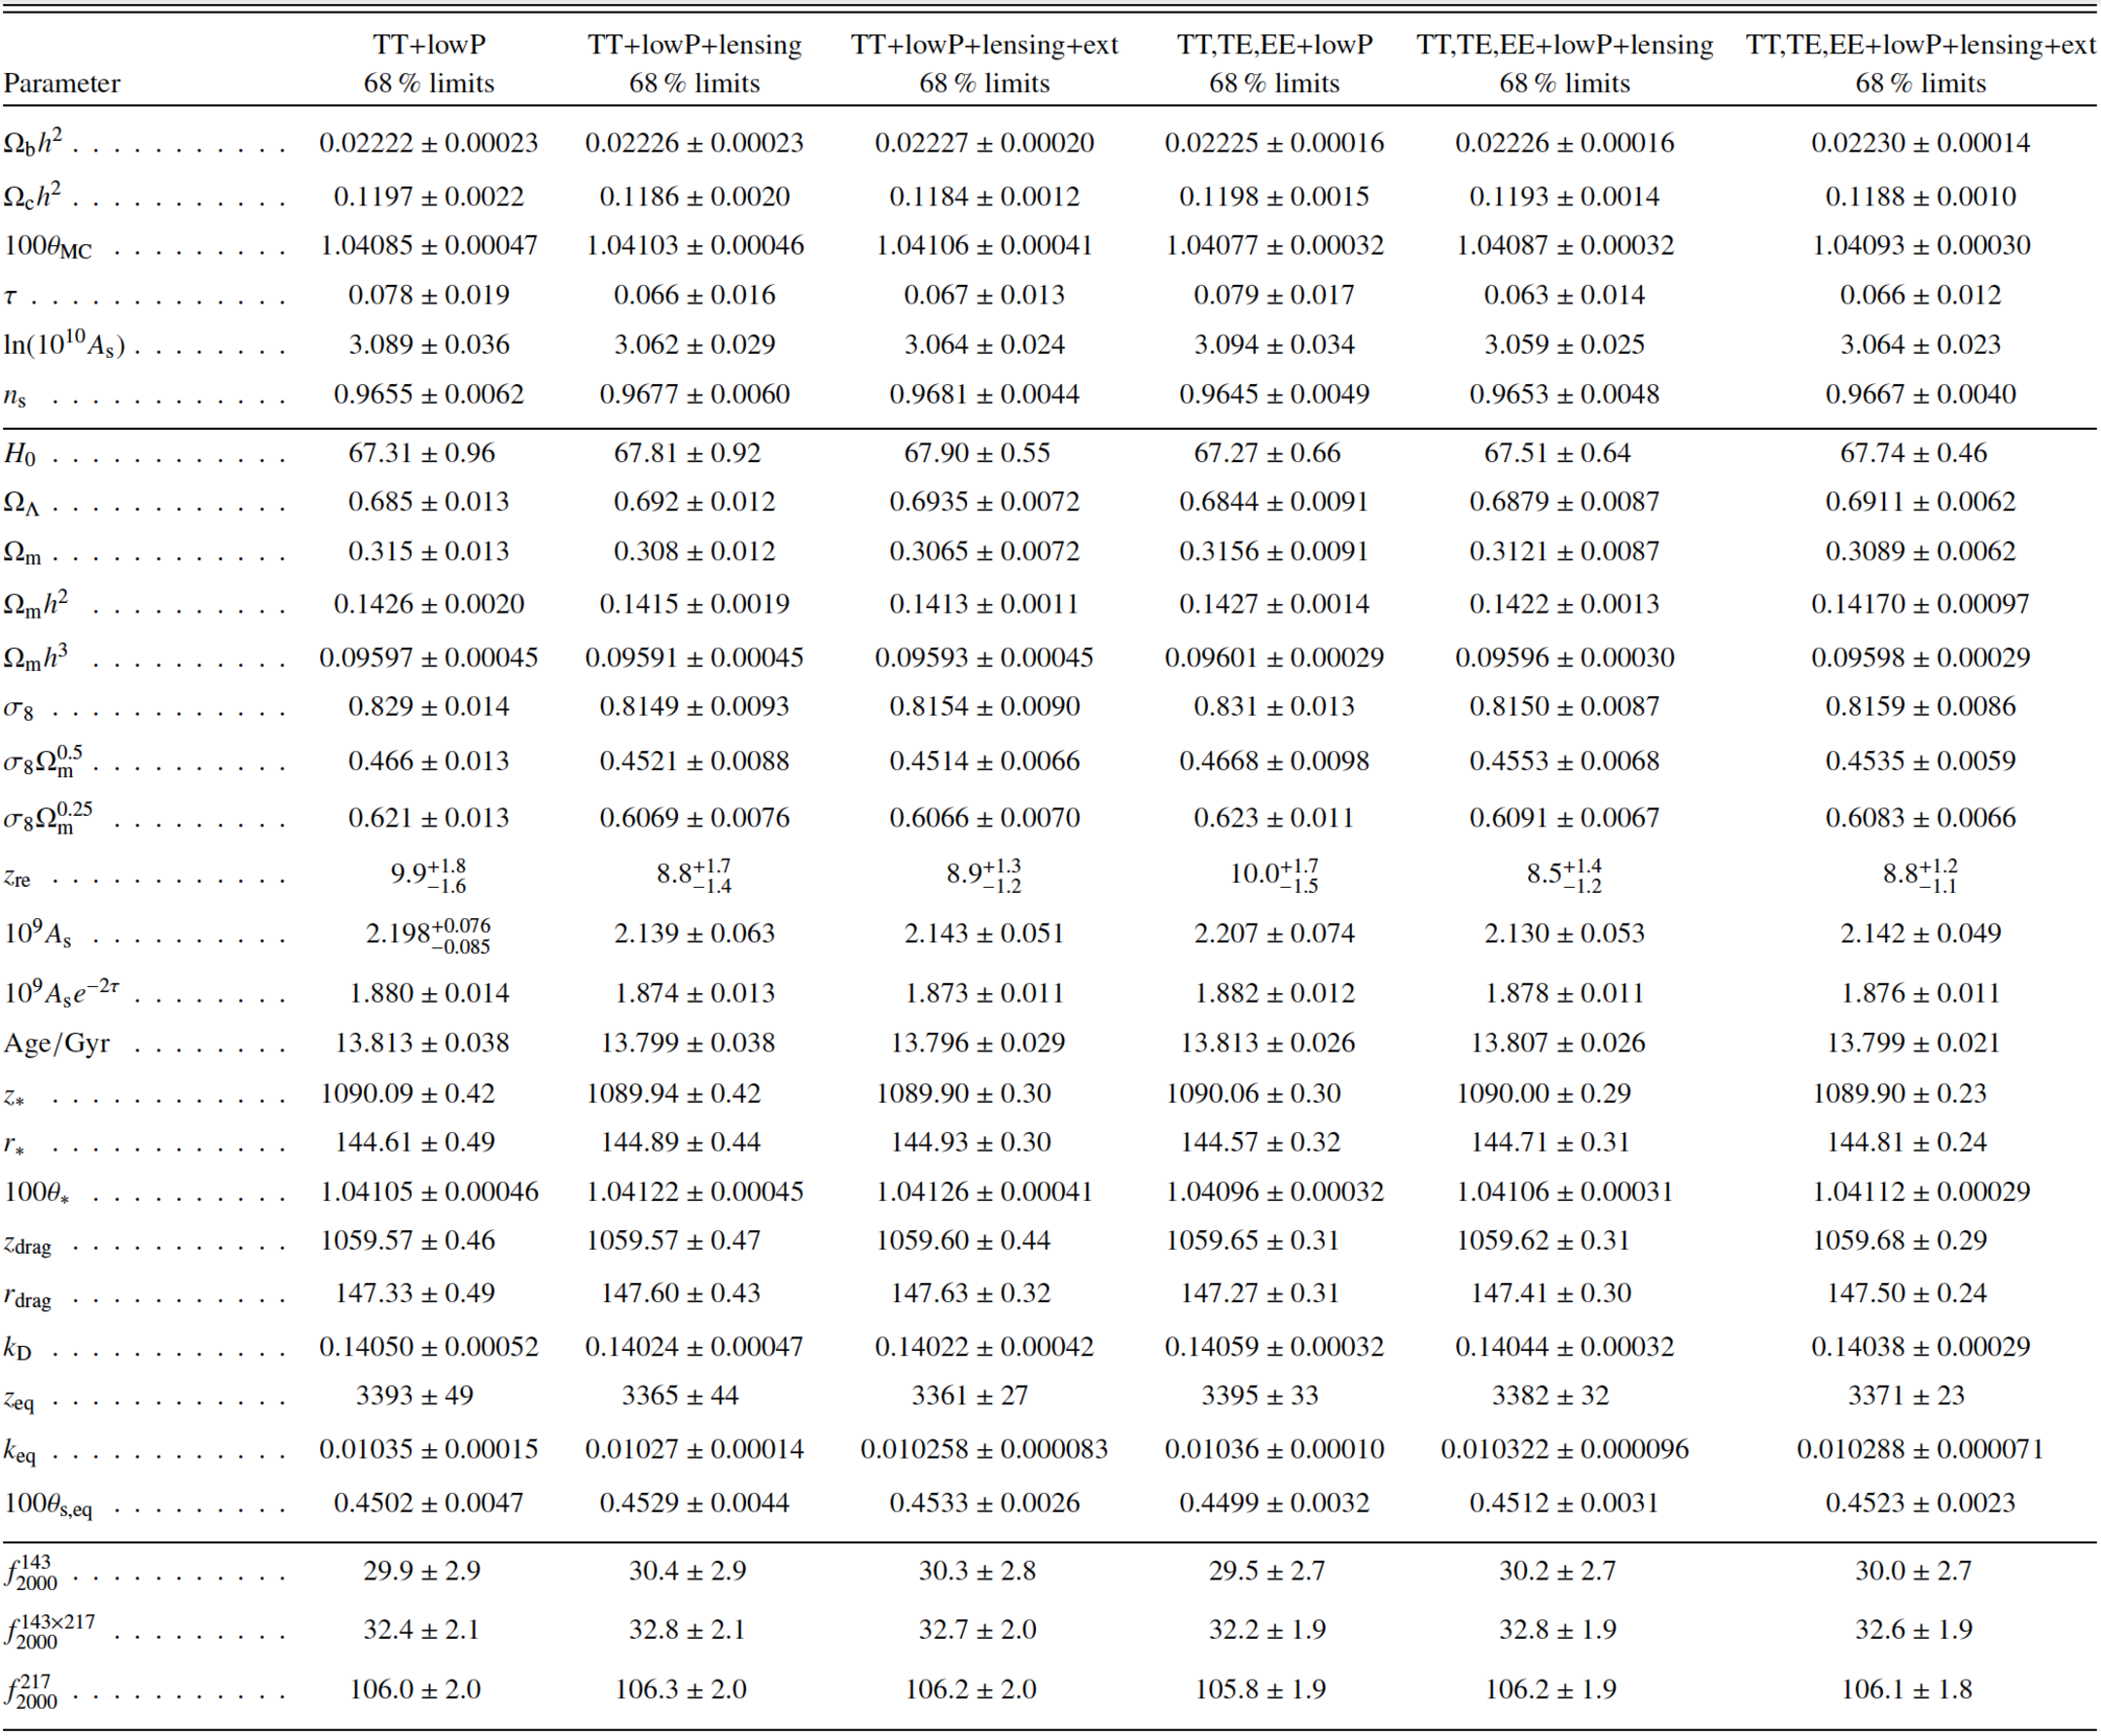
\includegraphics[width=.95\linewidth]{img/01/table_planck.pdf} 
        \caption{Determination des parametres cosmologiques par la colaboration Planck.}
 		\label{fig:planck_parameters}
\end{figure}

\citep{planck_collaboration_planck_2016}

\subsection{Energie noire $\Lambda$}

\subsubsection{Equation d'Einstein}

La notion d'un univers non statique a ete introduite par Einstein en 1917 en rapport avec ses travaux sur le relativité générale. 
Sa célèbre equation de champ décrivant le lien entre densité d'énergie et déformation de l'espace temps introduit la constante cosmologique $\Lambda$ representant 

Equation d'Einstein :
http://cdsads.u-strasbg.fr/abs/1915SPAW.......844E
\begin{equation}
R_{\mu\nu} = \frac{1}{2} g_{\mu\nu}R + \Lambda g_{\mu\nu}  = \kappa T_{\mu\nu}
\end{equation} 



Découverte de l'accélération de l'expansion de l'univers simultanément par 2 équipes :
Les 2 ont eue le prix nobel en 2011

\begin{itemize}
\item  Supernova Cosmology Project
 http://cdsads.u-strasbg.fr/abs/1999ApJ...517..565P
 
 \item  High-Z supernovae search team
http://cdsads.u-strasbg.fr/abs/1998AJ....116.1009R

\end{itemize}

quelques mois plus tard :
Première apparition du terme energie noire:
http://cdsads.u-strasbg.fr/abs/1999PhRvD..60h1301H



\subsubsection{ Équations de Friedmann }

 Recriture de l equation d'Einstein en considerant un univers homogene et isotrope.
 
 Alexandre Friedmann Über die Krümmung des Raumes, Zeitschrift für Physik 10, 377-386 (1922). Première écriture des équations de Friedmann, dans le cas d'une coubure spatiale positive. http://cdsads.u-strasbg.fr/abs/1922ZPhy...10..377F 
(de) Alexandre Friedmann, Über die Möglichkeit einer Welt mit konstanter negativer Krümmung des Raumes, Zeitschrift für Physik 21 326–332 (1924). Écriture des équations de Friedmann dans le cas d'une courbure spatiale négative. 
 
univers de Friedmann-Lemaître-Robertson-Walker  
http://dictionnaire.sensagent.leparisien.fr/%C3%89quations%20de%20Friedmann/fr-fr/
 
Équations de Friedmann : 
\begin{equation}
3 \left( \frac{H^2}{c^2} +\frac{K}{a^2} \right) = \frac{8 \pi G }{c^2} \rho
\label{eq:friedman1}
\end{equation}

\begin{equation}
-2 \frac{ \dot{H}}{c^2} -3 \frac{H^2}{c^2} -\frac{K}{a^2} = \frac{8 \pi G }{c^4 P}
\label{eq:friedman2}
\end{equation}

Eq. \ref{eq:friedman1} relie le taux d'expansion H, la courbure spatiale K et le facteur d'échelle a à la densité d'énergie $\rho$, 
Eq. \ref{eq:friedman2} relie la pression P à la dérivée temporelle du taux d'expansion
 
 
 
\begin{equation}
\frac{\dot{a}}{a} = H_0 \sqrt{ \Omega_{r,0} a^{-4} +  \Omega_{M,0} a^{-3} + \Omega_{K,0}a^{-2} + \Omega_{\lambda,0}  } 
\end{equation}


\begin{equation}
 \Omega_{i,0} = \frac{\rho_{i,0}}{\rho_{c,0}}
 \end{equation}

\begin{equation}
\rho_{c,0} = \frac{3H_0^2}{8\pi G}
 \end{equation}
 
 
\begin{equation}
 \Omega_{K,0} = 1 - \Omega_{r,0} - \Omega_{M,0} - \Omega_{\lambda,0} 
 \end{equation}

Univers plat
\begin{equation}
 \Omega_{K,0} = 0
 \end{equation}

\begin{equation}
\Omega_{\lambda,0} +  \Omega_{M,0} + \Omega_{r,0} =1
 \end{equation}




échelle gigaparsec\\
Facteur d'expansion


\begin{equation}
H=\frac{1}{a} \frac{da}{dt} = \frac{\dot{a}}{a}
\end{equation}

Metrique de Friedmann-Lemaître-Robertson-Walker (FLRW)


https://ned.ipac.caltech.edu/level5/Sept11/Norman/Norman2.html

\subsection{Matière noire CDM}

echelle mega parsec\\
gouverne la gravité\\
non collisionnelle\\


\begin{figure}[bth]
        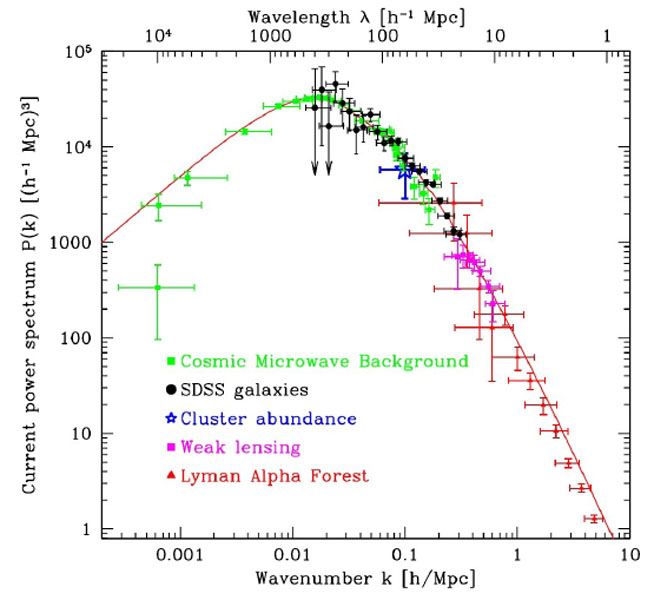
\includegraphics[width=.95\linewidth]{img/01/matter_power_spectrum.jpeg} 
        \caption{Spectre de puissance de distribution de la matière a grande échelle
        http://adsabs.harvard.edu/cgi-bin/bib_query?2004PhRvD..69j3501T}
 		\label{fig:matter_power_spectrum}
\end{figure}



\subsection{Baryon}

echelle kilo parsec
collisionnelle
interagit avec la radiation
La matière visible

\subsection{Radiation}

quasiment notre seul source d'information sur l'univers (plus vrai depuis les ondes gravitationnelles)
essentielle pour la reionization
seulement E>13.6 eV

\subsection{bilan}

plot en camembert avec les différents constituants






